\begin{figure}[t]
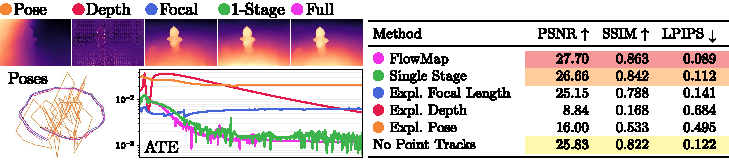
\includegraphics{figures/ablations/fig_ablations_pdf.pdf}



\caption{
\textbf{Ablations.}
We ablate the proposed feed-forward re-parameterizations of depth, pose, and intrinsics across all datasets.
We find that these reparameterizations are not only critical for high-quality downstream 3D Gaussian Splatting, but also lead to dramatically accelerated convergence, where FlowMap generally converges to high quality poses within a fraction of the optimization steps required for the ablated variants.
We further find that point tracks lead to a significant boost over optical flow alone (right).
See the supplemental document for more ablations.
\vspace{-10pt}
}
\label{fig:ablations}
\end{figure}

\section{Ablations and Analysis}
\label{sec:ablations}
We perform ablations to answer the following questions:
\setdefaultleftmargin{.5em}{0em}{}{}{}{}
\begin{itemize}
    \item \underline{Question 1:} Are FlowMap's reparameterizations of depth, pose, and intrinsics necessary, or do free variables perform equally well?
    \item \underline{Question 2:} Are point tracks critical to FlowMap's performance?
    \item \underline{Question 3:} Does self-supervised pre-training of the depth estimation and correspondence weight neural networks improve performance? 
\end{itemize}

\myparagraph{Parameterizations of Depth, Pose, and Camera Intrinsics (Q1)}

We compare the reparameterizations described in Sec.~\ref{sec:reparams} to direct, free-variable optimization of pose, depth, and intrinsics.
Fig.~\ref{fig:ablations} shows qualitative results and quantitative results averaged across 33 scenes.
We find that free-variable variants of FlowMap produce significantly worse reconstruction results and converge much more slowly, confirming that FlowMap's reparameterizations are crucial.

It is worth noting that often, explicitly optimizing a focal length produces high-quality results, as indicated by the relatively high performance of the ``Expl. Focal Length'' ablation.
In fact, given a good initialization, direct focal length regression produces slightly better results than the proposed focal length reparameterization alone on about 80 percent of scenes.
However, on about 20 percent of scenes, this approach falls into a local minimum and reconstruction fails catastrophically.
This justifies the approach FlowMap uses, where the first 1,000 optimization steps use a reparameterized focal length, which is then used to initialize an explicit focal length used for another 1,000 optimization steps.

We further highlight that FlowMap's reparameterizations are necessary to estimate poses and intrinsics in a single forward pass, which is crucial for the generalizable (pre-training) setting explored in Q3.

\myparagraph{Point Tracking (Q2)}
\label{point_track_exp}
While optical flow is only computed between adjacent frames, point track estimators can accurately track points across many frames. 
In Fig.~\ref{fig:ablations}, we show that FlowMap's novel view synthesis performance drops moderately when point tracks are disabled.
Qualitatively, we find that point tracks reduce drift for longer sequences, such as object-centric $360^\circ$ scenes.
This suggests that FlowMap will benefit from further improvements in point tracking methods.
We note that FlowMap's loss formulation is compatible with conventional correspondence methods (e.g. SIFT~\cite{sift} with RANSAC) and learned correspondences~\cite{sarlin20superglue}, which can be treated identically to point tracks.
FlowMap could also be extended to use conventional loop closure mechanisms, which would further reduce drift.

\myparagraph{Pre-training Depth and Correspondence Networks (Q3)}
\begin{figure*}[t!]
    \centering
    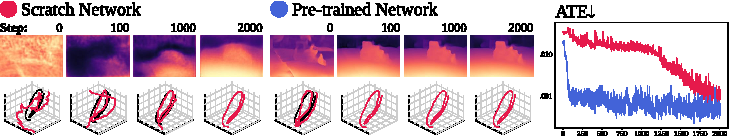
\includegraphics[width=\linewidth]{figures/init_vs_pretrain_pdf.pdf}
    \caption{\textbf{Effects of pretraining.} While a randomly initialized FlowMap network often provides accurate poses after optimization, pre-training leads to faster convergence and slightly improved poses. Here we plot depth estimates at specific optimization steps (left) as well as pose accuracy with respect to COLMAP during optimization (right). Randomly initialized FlowMap networks often require more than 20,000 steps to match the accuracy of a pre-trained initialization at 2,000 steps.}
    \label{fig:prior}
\end{figure*}

Since FlowMap is differentiable and provides gradients for any depth-estimating neural network, it is compatible with both randomly initialized neural networks and pre-trained priors.
Learned priors can come from optimization on many scenes, from existing depth estimation models, or from a combination of the two.
In practice, starting with a pre-trained prior leads to significantly faster convergence, as illustrated in Fig.~\ref{fig:prior}.
Note that pre-training and generalization are uniquely enabled by the proposed feed-forward reparameterizations of depth, focal length, and poses.
